\documentclass{article}

% Essential packages
\usepackage{graphicx}
\usepackage{tikz}
\usetikzlibrary{shapes,arrows.meta,calc,positioning,decorations.pathmorphing}
\usepackage{float}

% Define colors
\definecolor{MediumSlateBlue}{RGB}{123,104,238}

\begin{document}

% Figure 4: Model Schematic - Improved with correct forces and spacing
\begin{figure}[H]
    \centering
    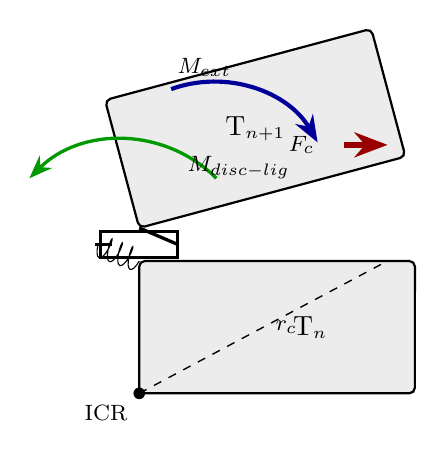
\begin{tikzpicture}[scale=1.4, every node/.style={font=\sffamily, font=\fontsize{8}{8}\selectfont}]
        
        % Setup with realistic proportions
        \def\w{2.5}      % Vertebra width
        \def\h{1.2}      % Vertebra height
        \def\phi{15}     % Rotation angle (used for positioning, not shown)
        
        % Base vertebra Tn
        \coordinate (ICR) at (0,0);
        \coordinate (TnBR) at ($(ICR) + (\w,0)$);
        \coordinate (TnTR) at ($(TnBR) + (0,\h)$);
        \coordinate (TnTL) at ($(ICR) + (0,\h)$);
        
        \fill[gray!15, draw=black, rounded corners=2pt, line width=0.8pt] (ICR) -- (TnBR) -- (TnTR) -- (TnTL) -- cycle;
        \node[font=\sffamily\bfseries, font=\fontsize{9}{9}] at ($(ICR)!0.5!(TnTR)+(0.3,0)$) {T$_n$};
        
        % Top vertebra Tn+1
        \coordinate (Tnp1BL) at ($(ICR)+(0,\h+0.3)$);
        \coordinate (Tnp1BR) at ($(Tnp1BL) + ({\w*cos(\phi)}, {\w*sin(\phi)})$);
        \coordinate (Tnp1TR) at ($(Tnp1BR) + ({-\h*sin(\phi)}, {\h*cos(\phi)})$);
        \coordinate (Tnp1TL) at ($(Tnp1BL) + ({-\h*sin(\phi)}, {\h*cos(\phi)})$);
        
        \fill[gray!15, draw=black, rounded corners=2pt, line width=0.8pt] (Tnp1BL) -- (Tnp1BR) -- (Tnp1TR) -- (Tnp1TL) -- cycle;
        \node[font=\sffamily\bfseries, font=\fontsize{9}{9}] at ($(Tnp1BL)!0.5!(Tnp1TR)$) {T$_{n+1}$};
        
        % ICR marker
        \fill[black] (ICR) circle (1.5pt);
        \node[below left=1pt] at (ICR) {ICR};
        
        % Moment arm r_c (dashed line) - back to original position
        \coordinate (cordPoint) at ($(TnTR)-(0.25,0)$);
        \draw[dashed, line width=0.5pt] (ICR) -- (cordPoint);
        \coordinate (rcMid) at ($(ICR)!0.5!(cordPoint)$);
        \node[right=1pt] at (rcMid) {$r_c$};
        
        % Spinal cord force vector (CORRECTED: pointing posteriorly)
        \coordinate (cordForceMid) at ($(cordPoint)!0.5!($(Tnp1TR)-(0.25,0)$)$);
        \draw[->, >=Stealth, line width=2pt, color=red!60!black] 
            ($(cordForceMid)-(0.2,0)$) -- ($(cordForceMid)+(0.2,0)$);
        \node[left=5pt] at ($(cordForceMid)-(0.25,0)$) {$F_c$};
        
        % Disc-ligament complex
        \coordinate (discStart) at (TnTL);
        \coordinate (discEnd) at (Tnp1BL);
        \coordinate (discMid) at ($(discStart)!0.5!(discEnd)$);
        
        % Spring-damper representation
        \draw[decorate, decoration={coil,aspect=0.25,segment length=4pt,amplitude=4pt}] 
        (discStart) -- ($(discMid)-(0.4,0)$);
        \draw[line width=1.2pt] ($(discMid)-(0.4,0)$) --++ (0.15,0);
        \draw[line width=1.2pt] ($(discMid)-(0.35,0.12)$) rectangle ++(0.7,0.24);
        \draw[line width=1.2pt] ($(discMid)+(0.35,0)$) -- (discEnd);
        
        % External moment M_ext (curved arrow) - moved more posteriorly
        \draw[->, >=Stealth, line width=1.5pt, color=blue!60!black] 
            ($(Tnp1TL)+(0.6,0.1)$) arc[start angle=110, end angle=30, radius=1.1];
        \node at ($(Tnp1TL)+(0.9,0.3)$) {$M_{\text{ext}}$};
        
        % Disc-ligament moment M_disc-lig (curved arrow) - moved more anteriorly
        \draw[->, >=Stealth, line width=1.2pt, color=green!60!black] 
            ($(discMid)+(0.7,0.6)$) arc[start angle=45, end angle=135, radius=1.2];
        \node at ($(discMid)+(0.9,0.7)$) {$M_{\text{disc-lig}}$};
        
    \end{tikzpicture}
    \caption{Lumped-parameter model schematic showing rigid vertebrae (T$_n$, T$_{n+1}$), disc-ligament spring-damper complex, and force vectors. The instantaneous center of rotation (ICR) and moment arm ($r_c$) are indicated. External moment ($M_{\text{ext}}$) drives flexion, resisted by disc-ligament moment ($M_{\text{disc-lig}}$) and spinal cord force ($F_c$). The model incorporates a torsional spring-damper system for the disc-ligament complex and a tensile element for the spinal cord, parameterized with material properties ($E_c = 0.3 \times 10^6$ Pa, $A_c = 3.2 \times 10^{-5}$ m$^2$, $L_0 = 0.102$ m) and geometric parameters ($r_c = 0.019$ m). The system's dynamic behavior is described by a second-order nonlinear ordinary differential equation that enables efficient simulation of dynamic strain evolution during traumatic hyperflexion events.}
    \label{fig:model_schematic}
\end{figure}

\end{document} 